% Laura Figueras
\documentclass[a4paper, 11pt]{article}
\usepackage[utf8]{inputenc} %alternativa: [latin1]
\usepackage[T1]{fontenc}
\usepackage[catalan]{babel} %alternativa: altres idiomes
\usepackage{amsmath, amssymb, amsthm}
\usepackage[margin=1in]{geometry}
\usepackage{hyperref}
\usepackage{enumerate}
\usepackage{array}
\usepackage{graphicx}
\usepackage{overpic}
\usepackage{epstopdf}
\usepackage{multicol}
\setlength{\parindent}{0cm}
\newtheorem*{definicio}{Definició}
\newtheorem*{obs}{Observació}
\newtheorem*{propietats}{Propietats}
\newtheorem*{prop}{Proposició}

\begin{document}
\title{Algebra lineal: Espais Vectorials}
\author{Laura Figueras}
\date{}
\maketitle

\thispagestyle{empty}
\setcounter{page}{0}


\begin{center}
	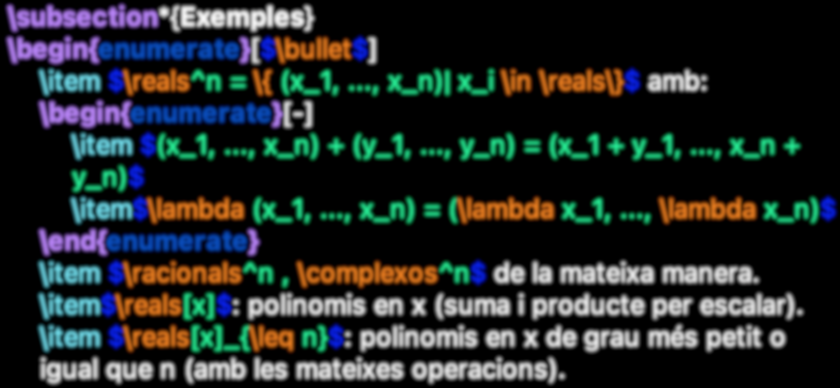
\includegraphics{LauraFigueras-1}
\end{center}

\newcommand{\Kcos}{\mathbb{K}}
\newcommand{\naturals}{\mathbb{N}}
\newcommand{\enters}{\mathbb{Z}}
\newcommand{\racionals}{\mathbb{Q}}
\newcommand{\reals}{\mathbb{R}}
\newcommand{\complexos}{\mathbb{C}}

\pagebreak

\section{Cos}
\begin{definicio}
	Un cos K (o bé $\Kcos$) és un conjunt amb dues operacions:
\end{definicio}

\begin{multicols}{2}
	Suma: 
\begin{align*}
	K \times K & \longrightarrow K \\
	\left( a, b \right) & \longmapsto a+b
\end{align*}

\columnbreak

Producte: 
\begin{align*}
	K \times K & \longrightarrow K \\
	\left( a, b \right) & \longmapsto a \cdot b
\end{align*}

\end{multicols}
Complint que:
\begin{multicols}{2}
\begin{enumerate}[$\bullet$]
	\item Propietat associativa: \\
	$\forall \, a, b, c \in K, \\
	(a+b)+c=a+(b+c)$
	\item Propietat commutativa: \\
	$\forall \, a, b \in K, \\
	a+b=b+a$
	\item Existeix un element neutre: \\
	$\exists \, 0 \in K $ tal que \\
	$a+0=a, \; \forall \; a \in K$
	\item Existència de l'oposat: \\
	$\forall \, a \in K, \; \exists \, b$ tal que \\
	$a+b=0$ ($"-a"$ oposat d'$a$)
\end{enumerate}
\columnbreak
\begin{enumerate}[$\bullet$]
	\item Propietat associativa: \\
	$\forall \, a, b, c \in K, \\
	(a \cdot b) \cdot c=a \cdot (b \cdot c)$
	\item Propietat commutativa: \\
	$\forall \, a, b \in K, \\
	a \cdot b=b \cdot a$
	\item Existeix un element neutre: \\
	$\exists \, 1 \in K,$ tal que \\
	$a \cdot 1=a, \forall a \in K$
	\item Existència de l'invers: \\
	$\forall \, a \not= 0, \; a \in K, \; \exists \, b$ tal que \\
	$a \cdot b=1$ ($"a^{-1}"$  invers d'$a$)
\end{enumerate}
\end{multicols}

\begin{multicols}{3}
\hphantom{hola}
\columnbreak
\begin{enumerate}[$\bullet$]
		\item  0 $\not$= 1 
		\item Propietat distributiva: \\
		$\forall \, a, b, c \in K,$\\
		$a \cdot (b+c)= ab+ac$ 
\end{enumerate}
\columnbreak
\hphantom{hola}
\end{multicols}

\subsection*{Exemples}
\begin{enumerate}[$\bullet$]
	\item $\racionals$, $\reals$ i $\complexos$ són cossos amb la suma i el producte que coneixem.
	\item $\enters$ amb la suma i producte que coneixem, no és un cos, ja que no té existència d'invers:
\begin{center}
	$2 \not =0$ i el 2 no té invers
\end{center}
\end{enumerate}

Com definir un cos nou: \\
$ K= \{0, 1\} \; + \: ,\;  \cdot$ \\
Definim la taula de la suma i la del producte:
\begin{table}[!ht]
	\centering
\begin{tabular}[c]{c | c c}
	$+$ & $0$ & $1$ \\
	\hline
	0 & 0 & 1 \\
	1 & 1 & 0 \\
\end{tabular}
\qquad \qquad
\begin{tabular}[c]{c | c c}
	$\cdot$ & 0 & 1 \\
	\hline
	0 & 0 & 0 \\
	1 & 0 & 1 \\
\end{tabular}
\end{table}

Ara definim un cos amb tres elements, amb les seves taules corresponents: \\
$K=\{0, 1, a\} \; + \: ,\;  \cdot$

\begin{table}[!ht]
	\centering
	\begin{tabular}[c]{c | c c c}
		+ & 0 & 1 & $a$ \\
		\hline
		0 & 0 & 1 & $a$ \\
		1 & 1 & $a$ & 0 \\
		$a$ & $a$ & 0 & 1 \\
	\end{tabular}
	\qquad \qquad
	\begin{tabular}[c]{c | c c c}
		$\cdot$ & 0 & 1 & $a$ \\
		\hline
		0 & 0 & 0 & 0 \\
		1 & 0 & 1 & $a$ \\
		$a$ & 0 & $a$ & 1 \\
	\end{tabular}
\end{table}

\pagebreak

\section{Espais Vectorials}
\begin{definicio}
	Fixem $\Kcos$ un cos. Diem que un conjunt E és un espai vectorial sobre $\Kcos$ (o un $\Kcos$-espai vectorial) si hi ha definides dues operacions:
\end{definicio}
\begin{multicols}{2}
	Suma de vectors:
	\begin{align*}
		E \times E & \longrightarrow E \\
		(\vec{u}, \vec{v}) & \longmapsto \vec{u} + \vec{v}
	\end{align*}

\columnbreak

	Multiplicació per escalar:
	\begin{align*}
		\Kcos \times E & \longrightarrow E \\
		(\lambda, \vec{v}) & \longmapsto \lambda \cdot \vec{v}
	\end{align*}
\end{multicols}
Complint que:
\begin{multicols}{2}
	\begin{enumerate}[$\bullet$]
		\item Associativa: \\
		$\forall \; \vec{u}, \vec{v}, \vec{w} \in E, \\
		(\vec{u} + \vec{v}) + \vec{w} = \vec{u} + (\vec{v} + \vec{w})$
		\item Commutativa: \\
		$ \forall \; \vec{u}, \vec{v} \in E, \\
		\vec{u} + \vec{v} = \vec{v} + \vec{u}$
		\item Element neutre: \\
		vector zero $\vec{0} \\
		\vec{u} + \vec{0} = \vec{u}, \; \forall \; \vec{u} \in E$
		\item Element oposat: \\
		$\forall \; \vec{u} \in E, \;  \exists \; \vec{v}$ \\
		tal que $\vec{u} + \vec{v} = \vec{0}$
	\end{enumerate}

\columnbreak

	\begin{enumerate}[$\bullet$]
		\item Associativa mixta: \\
		$\forall \; \lambda, \mu \in \Kcos, \; \forall \; \vec{u} \in E, \\
		\lambda \cdot (\mu \cdot \vec{u}) = (\lambda \cdot \mu) \cdot \vec{u}$
		\item Distributiva (1) \\
		$\forall \; \lambda, \mu \in \Kcos, \; \forall \; \vec{u} \in E, \\
		(\lambda + \mu) \cdot \vec{u} = \lambda \vec{u} + \mu \vec{u}$
		\item Distributiva (2) \\
		$\forall \; \lambda \in \Kcos, \; \forall \; \vec{u}, \vec{v} \in E, \\
		\lambda(\vec{u}+\vec{v}) = \lambda \vec{u} + \lambda \vec{v}$
		\item Unitat: \\
		$\forall \; \vec{u} \in E, \\
		1 \cdot \vec{u} = \vec{u}$
	\end{enumerate}
\end{multicols}
Anomenem vectors als elements de E i escalars als elements de $\Kcos$.

\subsection*{Exemples}
\begin{enumerate}[$\bullet$]
	\item $\reals^n = \{ (x_1, ..., x_n) \; | \; x_i \in \reals\}$ amb:
	\begin{enumerate}[-]
		\item $(x_1, ..., x_n) + (y_1, ..., y_n) = (x_1 + y_1, ..., x_n + y_n)$
		\item$\lambda (x_1, ..., x_n) = (\lambda x_1, ..., \lambda x_n)$
	\end{enumerate}
	\item $\racionals^n , \complexos^n$ de la mateixa manera.
	\item$\reals[x]$: polinomis en x (suma i producte per escalar).
	\item $\reals[x]_{\leq n}$: polinomis en x de grau més petit o igual que n (amb les mateixes operacions).
\end{enumerate}
\begin{obs}
A l'estructura d'espai vectorial no podem multiplicar polinomis.
\end{obs}
\begin{enumerate}[$\bullet$]
	\item $M_{m \times n} (\reals)$, suma de matrius i multiplicació per un escalar, també és un espai vectorial.
\end{enumerate}

\begin{propietats}\label{propietats}
	E espai vectorial sobre $\Kcos$:
\end{propietats}
\begin{enumerate}[A)]
	\item El vector $\vec{0}$ és únic.
	\item $\forall \; \vec{u} \in$ E, el vector oposat és únic.
	\item $0 \cdot \vec{u} = \vec{0}, \; \forall \, \vec{u} \in E$
	\item $\lambda \cdot \vec{0} = \vec{0}, \; \forall \, \lambda \in \Kcos$
	\item $\lambda \cdot \vec{u} = \vec{0} \iff (\lambda = 0 \; \cup \; \vec{u} = \vec{0})$
	\item$-\vec{u} = (-1) \cdot \vec{u}$
\end{enumerate}
Ara demostrarem algunes de les $\text{propietats}^{\ref{propietats}}$ mencionades anteriorment.
\begin{proof}
	Començarem per l'apartat A):
	
	Suposem $\vec{0}$ i $\vec{0'}$ dos elements neutres per la suma i veiem que, al sumar-los, passa el següent:
	\begin{equation*}
		\vec{0}=\vec{0}+\vec{0'}=\vec{0'} \\
	\end{equation*}
	Per una banda, si considerem $\vec{0'}$ l'element neutre, el resultat seria el vector $\vec{0}$. Per altra banda, si el que considerem neutre és el $\vec{0}$, el resultat seria el vector $\vec{0'}$. Per tant queda que:
	\begin{equation*}
		\vec{0}=\vec{0'}
	\end{equation*}
\end{proof}
\begin{proof}
	Ara demostrarem l'apartat C):
	
	Sigui $\vec{u}$ un vector i -$\vec{u}$ el seu oposat:
	\begin{equation*}
		0 \cdot \vec{u} + \vec{u} = (0+1) \cdot \vec{u} = \vec{u}
	\end{equation*}
	Ens queda que $0\cdot\vec{u}+\vec{u}=\vec{u}$, llavors si sumem el vector oposat de $\vec{u}$, ens queda que:
	\begin{align*}
		0\cdot\vec{u} + \vec{u} + (-\vec{u}) &= \vec{u} + (-\vec{u}) \\
		0\cdot\vec{u}&=\vec{0}
	\end{align*}
\end{proof}

\subsection*{Exemples d'espais vectorials}
A conjunt i E un $\Kcos$-espai vectorial:
\begin{align*}
	f: A & \longrightarrow E  \qquad \qquad &g: A &\longrightarrow E\\
	 a & \longmapsto f(a) \qquad \qquad & a& \longmapsto g(a)
\end{align*}
Tenim que:
\begin{align*}
	(f+g): A & \longrightarrow E  \qquad \qquad &(\lambda f): A &\longrightarrow E \\
	a & \longmapsto f(a)+g(a) \qquad \qquad & a& \longmapsto \lambda f(a)
\end{align*}
D'aquesta manera, les aplicacions d'A en E, tenen estructura d'espai vectorial.

\medskip

Un cas particular:
$\begin{cases}
	A=\reals \\
	E=\reals \text{ com } \reals \text{-espai vectorial}
\end{cases}$
\begin{equation}
	\{f: \reals \longrightarrow \reals\}
\end{equation}
\begin{equation}
	\{f: \reals \longrightarrow \reals\ | \: \text{f és contínua}\}
\end{equation}
\begin{equation}
	\{f: \reals \longrightarrow \reals\ | \: \text{f és derivable}\}
\end{equation}

\section{Subespais vectorials}
\begin{definicio}
	Si E és un $\Kcos$-espai vectorial, diem que $F \subseteq E$ un subconjunt no buit és un subespai si es compleix:
\end{definicio}
\begin{enumerate}[(i)]\label{subespai}
	\item $\forall \; \vec{u}, \vec{v} \in F, \; \vec{u}+\vec{v} \in F$
	\item $\forall \; \vec{u} \in F$ i  $\forall \; \lambda \in \Kcos, \; \lambda\vec{u} \in F $
\end{enumerate}
\begin{obs}
	Si F $\subseteq$ E és un subespai, $\vec{0}$ $\in$ F:
\end{obs}
\begin{equation*}
	F \not = \varnothing 
	\iff 
	\begin{cases}
		\exists \; \vec{u} \in F \\
		0 \in \Kcos
	\end{cases}
	\overset{(ii)}{\iff}
	\;
	\begin{cases}
		0 \cdot \vec{u} \in F \\
		0 \cdot \vec{u} = \vec{0}
	\end{cases}
\end{equation*}

\begin{prop}\label{prop}
	Si $E$ és un $\Kcos$-espai vectorial i $F \subseteq E$ és un conjunt no buit, llavors $F$ és un subespai si i només si:
\end{prop}
\begin{enumerate}[(a)]
	\item $\forall \; \vec{u}, \vec{v} \in F$  i  $\forall \; \lambda, \mu \in \Kcos$, tenim que $\lambda\vec{u}+\mu\vec{v} \in F$
\end{enumerate}
\begin{proof}
	Demostrem que $(i)+(ii)\iff(a)$:
	\begin{enumerate}[$\Rightarrow$]
		\item Siguin:
		
		$\begin{cases}
			\vec{u}, \vec{v} \in F \\
			\lambda, \mu \in \Kcos
		\end{cases}$
		
		Per la segona propietat de la definició de $\text{subespais vectorials}^{\ref{subespai}}$, sabem que:
		
		\begin{equation*}
			\begin{cases}
				\lambda\vec{u} \in F \\
				\mu\vec{v} \in F
			\end{cases}
			\overset{(i)}{\Longrightarrow}
			\lambda\vec{u}+\mu\vec{v} \in F
		\end{equation*}
	\end{enumerate}
	\begin{enumerate}[$\Leftarrow$]
		\item Sigui $\vec{u}, \vec{v} \in F$, per la propietat de la $\text{proposició}^{\ref{prop}}$, sabem que $\vec{u}+\vec{v}\in F$ quan $\lambda=\mu=0$.
		
		Ara, veiem la segona propietat. Sigui $\vec{u}\in F, \; \lambda\in\Kcos$. Per la propietat de la proposició, sabem que $\lambda\vec{u} \in F$ quan $\mu=0$.
	\end{enumerate}
\end{proof}

\subsection*{Exemples}
\begin{enumerate}[$\bullet$]
	\item E qualsevol, F=$\{\vec{0}\}$
	\item Si $\{\vec{v_1}, \vec{v_2}, ..., \vec{v_n}\} \subset$ E, considerem:
	\begin{equation*}
		\langle\vec{v_1}, \vec{v_2}, ..., \vec{v_n}\rangle = \{\lambda_1\cdot\vec{v_1} + \lambda_2\cdot\vec{v_2} + ... + \lambda_n\cdot\vec{v_n} \: | \: \lambda_i \in \Kcos, \; i=1...n\}
	\end{equation*}
	Vegem que és un subespai:
	\begin{enumerate}[(i)]
		\item $\vec{u}=\lambda_1\vec{v_1} + \lambda_2\vec{v_2} + ... + \lambda_n\vec{v_n} \quad \in \quad \langle\vec{v_1}, \vec{v_2}, ..., \vec{v_n}\rangle$
		
		$\vec{v}=\mu_1\vec{v_1} + \mu_2\vec{v_2} + ... + \mu_n\vec{v_n} \quad \in \quad \langle\vec{v_1}, \vec{v_2}, ..., \vec{v_n}\rangle$
		
		\bigskip
		
		$\vec{u}+\vec{v}=(\lambda_1+\mu_1)\vec{v_1} + (\lambda_2\mu_2)\vec{v_2} + ... + (\lambda_n\mu_n)\vec{v_n} \quad \in \quad \langle\vec{v_1}, \vec{v_2}, ..., \vec{v_n}\rangle$
		
		\medskip
		
		\item $\vec{u} = \lambda_1\vec{v_1} + \lambda_2\vec{v_2} + ... +\lambda_n\vec{v_n}, \qquad \mu \in \Kcos$
		
		$\mu \vec{u} = (\mu \lambda_1)\vec{v_1} + (\mu \lambda_2)\vec{v_2} + ... + (\mu \lambda_n)\vec{v_n} \; \in \langle \vec{v_1}, \vec{v_2}, ..., \vec{v_n} \rangle$
		
		\medskip
		
		\begin{enumerate}[$\diamond$]
			\item $E=M_2(\reals), \; F = \langle \left( \begin{smallmatrix}
				1 & 0 \\ 0 & 0
			\end{smallmatrix} \right), \,
		\left( \begin{smallmatrix}
			0 & 1 \\ 0 & 0
		\end{smallmatrix} \right), \, 
		\left( \begin{smallmatrix}
		0 & 1 \\ 1 & 0
		\end{smallmatrix} \right) \rangle$
		
		\medskip
		
		$F = \{ \lambda_1 \left( \begin{smallmatrix}
			1 & 0 \\ 0 & 0
		\end{smallmatrix} \right) + \lambda_2 \left( \begin{smallmatrix}
		0 & 0 \\ 0 & 1
		\end{smallmatrix} \right) + \lambda_3 \left( \begin{smallmatrix}
		0 & 1 \\ 1 & 0
		\end{smallmatrix} \right) \; | \; \lambda_1, \lambda_2, 	\lambda_3 \in \reals \} $
		
		\medskip
		
		$=\{ \left( \begin{smallmatrix}
			\lambda_1 & \lambda_3 \\ \lambda_3 & \lambda_2
		\end{smallmatrix} \right) \; | \; \lambda_1, \lambda_2, \lambda_3 \in \reals\}$ = matrius simètriques 2 $\times$ 2
		
		\medskip
		
		$F= \{ \left( \begin{smallmatrix}
			a & b \\ c & d
		\end{smallmatrix} \right) \; | \; b-c=0\}$
		
		\medskip
		
		\item Solucions d'equacions lineals homogenies:
		
		Suposem A una matriu m$\times$n  i $X= \left( \begin{smallmatrix}
			x_1 \\
			\vdots \\
			x_n
		\end{smallmatrix} \right)$ incògnites.
		
		\medskip
		
		$AX=\left( \begin{smallmatrix}
			0 \\
			\vdots \\
			0
		\end{smallmatrix} \right)$ sistema d'equacions homogenia.
		\end{enumerate}
	\end{enumerate}
\begin{obs}
	Les solucions d'aquest sistema són subespais de $\Kcos^n$
\end{obs}
\begin{proof} Hi ha tres casos:
	
	\begin{enumerate}[$\cdot$]
		\item $X= \left( \begin{smallmatrix}
			0 \\
			\vdots \\
			0
		\end{smallmatrix} \right) $ és una solució, solucions $\not = \varnothing$
	
		\item $\begin{cases}
			X= \left( \begin{smallmatrix}
				x_1 \\
				\vdots \\
				x_n
			\end{smallmatrix} \right)   \text{solució}  \qquad A (X+Y) \overset{?}{=} \left( \begin{smallmatrix}
			0 \\
			\vdots \\
			0
		\end{smallmatrix} \right) \\
			Y= \left( \begin{smallmatrix}
				y_1 \\
				\vdots \\
				y_n
			\end{smallmatrix} \right)  \text{solució} \qquad AX + AY = \left( \begin{smallmatrix}
			0 \\
			\vdots \\
			0
			\end{smallmatrix} \right) + \left( \begin{smallmatrix}
			0 \\
			\vdots \\
			0
			\end{smallmatrix} \right) = \left( \begin{smallmatrix}
			0 \\
			\vdots \\
			0
			\end{smallmatrix} \right)
		\end{cases}$
		
		\item $\begin{cases}
			X \text{solució} \qquad A(\lambda X) \overset{?}{=} \left( \begin{smallmatrix}
				0 \\
				\vdots \\
				0
			\end{smallmatrix} \right) \\
		
		\lambda \in \Kcos \qquad \lambda (AX)= \lambda \left( \begin{smallmatrix}
			0 \\
			\vdots \\
			0
		\end{smallmatrix} \right) = \left( \begin{smallmatrix}
		0 \\
		\vdots \\
		0
	\end{smallmatrix} \right)
		\end{cases}$
	\end{enumerate}
\end{proof}
\end{enumerate}
\end{document}


